\documentclass[10pt,twocolumn]{article}

% use the oxycomps style file
\usepackage{oxycomps}
\usepackage{subcaption} 

% usage: \fixme[comments describing issue]{text to be fixed}
% define \fixme as not doing anything special
\newcommand{\fixme}[2][]{#2}
% overwrite it so it shows up as red
\renewcommand{\fixme}[2][]{\textcolor{red}{#2}}
% overwrite it again so related text shows as footnotes
%\renewcommand{\fixme}[2][]{\textcolor{red}{#2\footnote{#1}}}

% read references.bib for the bibtex data
\bibliography{references}

% include metadata in the generated pdf file
\pdfinfo{
    /Title (StellarSim: A Computational Framework for Star Cluster Evolution)
    /Author (Student Name)}

% set the title and author information
\title{StellarSim: A Computational Framework for Star Cluster Evolution}
\author{Bernie Cassidy}
\affiliation{Occidental College}
\email{bcassidy@oxy.edu}

\begin{document}

\maketitle

\section{Abstract}

This paper presents the development and evaluation of a simulation framework, StellarSim, designed to model the evolution of star clusters. The framework integrates gravitational dynamics, stellar evolution, and tidal effects within the AMUSE (Astrophysical Multipurpose Software Environment) platform. The simulation models the interactions between stars using the Hermite N-body algorithm and tracks stellar evolution through the SeBa code. Key parameters such as mass loss, density profiles, and truncation radius are evaluated over time to assess the cluster's stability and evolution. The project utilizes high-performance computing resources at Occidental College's Bletchley cluster to run simulations with 1,000 stars over 100 million years. The results demonstrate that the simulation captures expected trends in mass loss and density evolution, validating the chosen methodologies. Ethical considerations, particularly regarding the use of AI tools in the coding process, are discussed, highlighting the importance of maintaining scientific integrity and transparency. This paper lays the foundation for further exploration into more detailed simulations of star cluster dynamics.

\section{Introduction and Problem Context}
Star clusters are gravitationally bound collections of stars that form from a common molecular cloud around the same time. These systems, which can range from a few hundred to millions of stars, offer a unique opportunity to study stellar evolution in a controlled environment where all stars are of the same age and chemical composition. Clusters are categorized into open clusters, which are younger and less dense, and globular clusters, which are older and densely packed. These groupings are significant for astronomers because they provide snapshots of stellar evolution under a variety of conditions, from the earliest stages of star formation to the eventual dispersion of the cluster into the galactic field \cite{Takahashi2000}.

Despite their importance, star clusters are difficult to study directly. Observations of cluster dynamics are hindered by several factors, particularly the density of clusters' cores and the length of the timescales on which they evolve. The high density of stars in the cluster's core leads to overlapping observations, making it challenging to discern individual stellar properties, and cluster lifetimes span hundreds of millions to billions of years, far exceeding the timescales available for direct observation or experimental study.\cite{clusters}

Given these difficulties, computational simulations are needed to study the long-term evolution of star clusters. Numerical models allow researchers to replicate the physical processes governing clusters, such as gravitational interactions, stellar evolution, and the galactic tidal cutoff, which causes individual stars to escape the cluster due to the galaxy's tidal influence. By tracking changes in the cluster's properties over time, simulations provide insights that are unattainable through direct observation \cite{whitehead2013amuse}.

This project, StellarSim, seeks to address these challenges by implementing a simulation of star clusters using the Astrophysical Multipurpose Software Environment (AMUSE). AMUSE is an open-source Python framework designed for astrophysical simulations, integrating various numerical solvers for gravity, stellar evolution, and hydrodynamics \cite{pelupessy2013amuse}. StellarSim focuses on three critical aspects of cluster evolution: gravitational interactions, stellar evolution, and galactic tidal effects. The gravitational forces between stars are modeled using N-body simulations, which compute the positions and velocities of stars over time. Individual stars are evolved using predefined stellar tracks, capturing changes in properties like mass, temperature, and luminosity. The simulation also models the galactic tidal force by attempting to determine the cluster's truncation radius—the distance beyond which stars experience more force from the center of the galaxy in which the cluster is situated than from the cluster's center of mass \cite{portegies2013multiphysics}.

    \begin{figure}
        \centering
            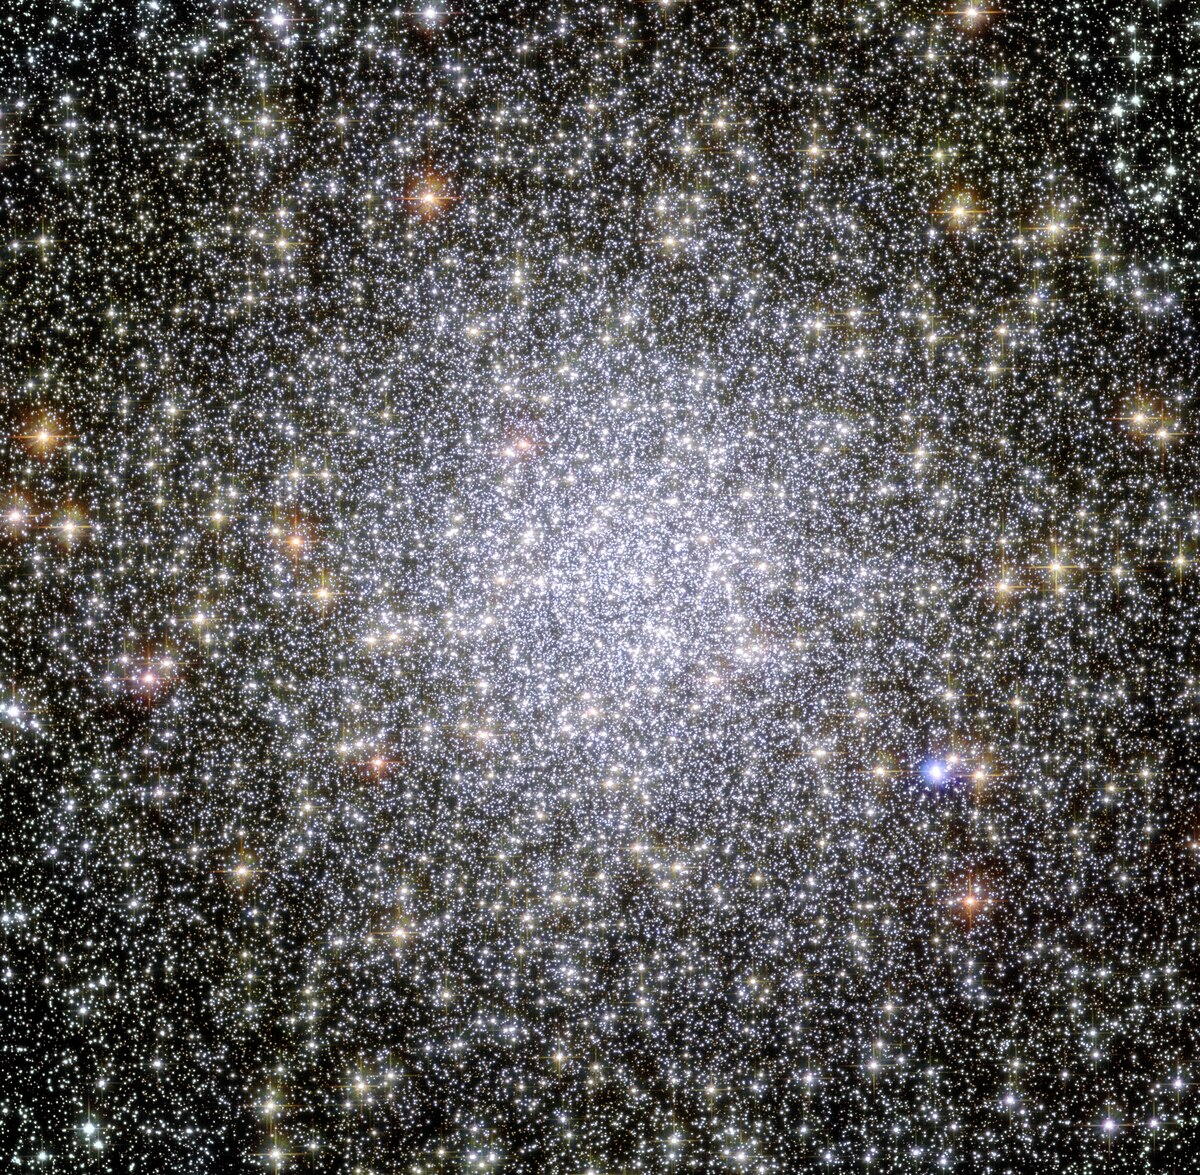
\includegraphics[width=0.75\linewidth]{47tuc.jpg}
            \caption{47 Tucanae, a star cluster}
            \label{fig:47tuc, a star cluster visible with the naked eye}
    \end{figure}


The simulation tracks several key metrics, including the cluster's total mass, the mass of stars escaping the cluster, and the density distribution over time. These metrics are critical for evaluating the cluster's stability, understanding the mechanisms driving its evolution, and comparing results with observational data. StellarSim provides a framework for studying and visualizing star cluster dynamics and evolution, contributing to a deeper understanding of stellar systems.

\section{Technical Background}
Modeling star clusters requires an interdisciplinary approach that integrates astrophysical concepts, numerical methods, and computational optimization. This section outlines the key technical components of the StellarSim framework, including the underlying astrophysical models, numerical solvers, and considerations of computational complexity.

\subsection{Astrophysical Multipurpose Software Environment (AMUSE)}
StellarSim is built on the Astrophysical Multipurpose Software Environment (AMUSE), an open-source Python framework for astrophysical simulations \cite{portegies2018amuse}. AMUSE facilitates the integration of diverse solvers for gravity, stellar evolution, and hydrodynamics, making it an ideal choice for star cluster modeling. The modularity of AMUSE allows users to experiment with different solvers for the same physical process, enabling comparisons and optimizations tailored to specific simulations. This was very helpful for the project because I was able to try different solvers and functions that produced initial conditions before selecting the ones that worked the best.

\subsection{N-Body Gravitational Solvers}
The gravitational dynamics of the cluster are computed using the Hermite algorithm, a N-body integrator designed for high precision. N-body simulations model the gravitational interactions between stars by solving the equations of motion for each star under the influence of every other star. The Hermite integrator is particularly suitable for star cluster dynamics due to its adaptive timestep mechanism, which ensures computational efficiency without sacrificing accuracy. The computational complexity of N-body simulations is $O(N^2)$, where $N$ is the number of stars in the cluster. This quadratic scaling arises from the pairwise force calculations required for each star at every timestep. As a result, the simulation of large clusters is computationally expensive, necessitating efficient algorithms and, in some cases, the use of parallel computing resources \cite{Hut1995}.

\subsection{Stellar Evolution Codes}
The SeBa algorithm is used to model the individual evolution of stars within the cluster \cite{PortegiesZwart1996}. SeBa tracks changes in stellar properties, such as mass, radius, temperature, and luminosity, based on predefined evolutionary tracks. SeBa also accounts for processes like mass loss due to stellar winds and supernovae, which are critical for understanding the overall evolution of the cluster. SeBa is computationally efficient, as it interpolates stellar evolution tracks rather than solving the full set of stellar structure equations for each star.

\subsection{Tidal Cutoff and Truncation Radius}
Star clusters are subject to the tidal influence of their host galaxy, which defines a boundary known as the truncation radius. Beyond this radius, the galaxy’s gravitational forces overpower the cluster’s self-gravity, causing stars to escape. StellarSim models the tidal cutoff by iteratively computing the cluster's density profile and identifying the radius where the density approaches zero. This boundary evolves over time as stars migrate within the cluster and escape its gravitational influence \cite{Takahashi2000}.

\subsection{King Model and Kroupa Initial Mass Function}
The Kroupa Initial Mass Function (IMF) is a widely used empirical model that describes the distribution of stellar masses in a population of stars, typically in young star clusters \cite{Kroupa2001}. It is a piecewise function that approximates the probability of a star forming at a given mass, with a slope of -1.3 for stars with masses between 0.1 and 0.5 solar masses, and a steeper slope of -2.3 for stars with masses greater than 0.5 solar masses. This mass distribution reflects the observed stellar populations in various star-forming regions and ensures that the simulated cluster's mass spectrum is realistic. The King Model is a widely used model for simulating the spatial distribution of stars in a star cluster \cite{king1966}. It describes a cluster with a centrally concentrated distribution of stars, characterized by a parameter $w_0$ that sets the cluster's concentration. A King model with $w_0=7$, as used in this simulation, represents a moderately concentrated cluster similar to a globular cluster, while $w_0=3$, also used, would represent an open cluster. This model takes into account the gravitational potential of the cluster and the balance between the stars' kinetic energy and the cluster's gravitational binding energy, providing a realistic initial distribution of stars for simulating the cluster's evolution.

\subsection{Visualization and Data Tracking}
The simulation tracks the position, mass, and stellar type of each star over time, providing a detailed record of the cluster’s evolution. Key metrics, such as the cluster’s total mass and density profile, are visualized through graphs and animations. For example, 3D animations of star positions illustrate the dynamical behavior of the cluster, while density profiles highlight how mass becomes less concentrated at the center over time. For an example of the 3D visualization used for this project, see \ref{fig:One frame of a 3D visualization of a star cluster}.

    \begin{figure}
            \centering
            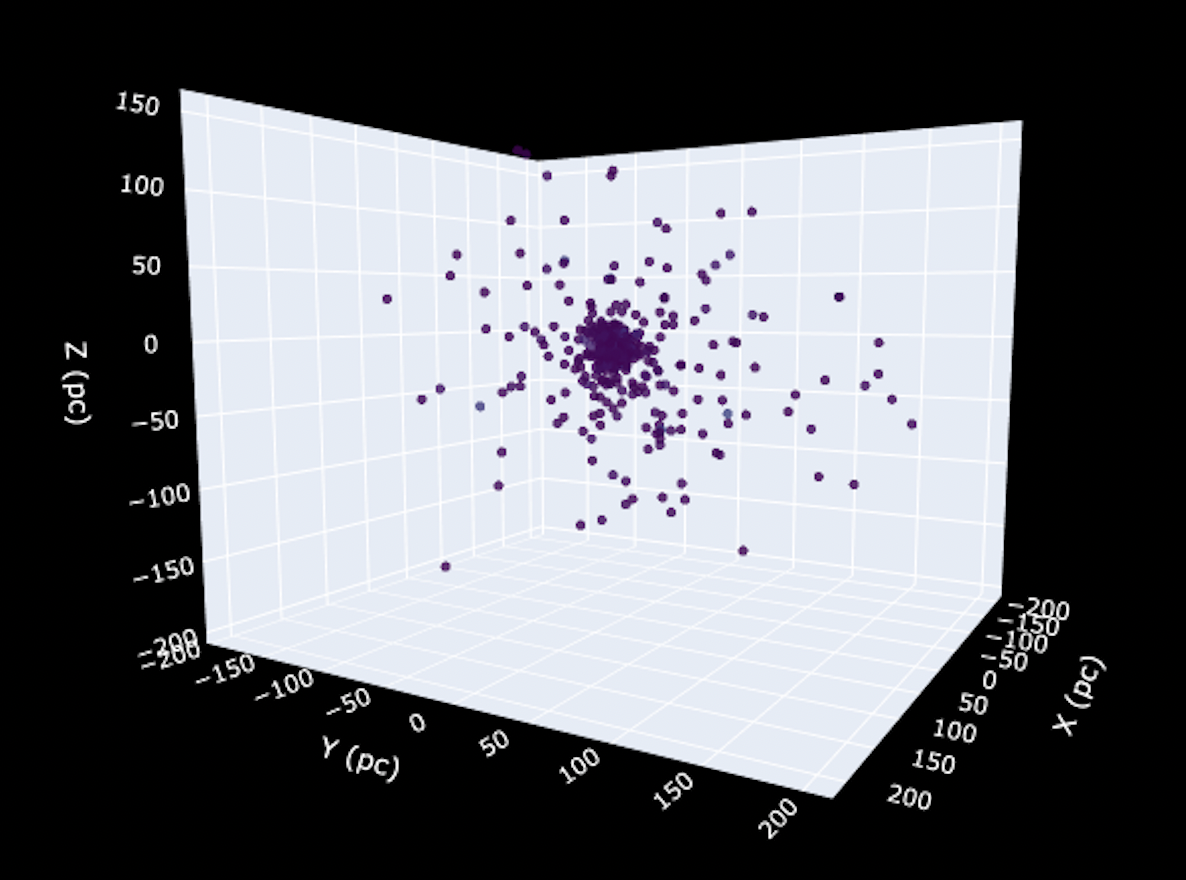
\includegraphics[width=\linewidth]{3DAnimation.png}
            \caption{One frame of a 3D visualization of a star cluster}
            \label{fig:One frame of a 3D visualization of a star cluster}
    \end{figure}


\subsection{Summary}
StellarSim combines several algorithms, including some that were taken from AMUSE and some that I wrote, to provide a robust simulation of star clusters. Although the simulation poses significant computational challenges due to the large number of interacting particles and the need for high temporal resolution, it successfully balances the physical accuracy needed for astrophysical research with the computational efficiency required for practical application \cite{portegies2009newastronomy}.

\section{Prior Work}

\subsection{Takahashi and Zwart (2000)}
Simulating the evolution of star clusters is a well-established area of research in astrophysics, with a significant amount of prior work focusing on understanding the underlying dynamics, the effects of galactic tidal forces, and the role of stellar evolution. Several key studies and simulation frameworks have contributed to the development of models for star clusters, which provide context and inform the approach used in this project.

One notable study is by Takahashi and Zwart (2000), which investigated the evolution of star clusters under galactic tidal forces. The authors used N-body simulations to model the interaction between stars and the gravitational influence of the galaxy, examining how these tidal forces affect the cluster's structure over time. Their findings provided valuable insights into the role of the galactic environment on cluster evolution, particularly in terms of mass loss and the formation of tidal tails. This work helped establish the importance of including galactic tidal forces in any model of star cluster evolution, a consideration that was also central to this project \cite{Takahashi2000}.

\subsection{Whitehead et al. (2013)}
Another important contribution comes from Whitehead et al. (2013), who explored the use of the AMUSE (Astrophysical Multipurpose Software Environment) framework to simulate star clusters. Their work focused on using the AMUSE software to model the interplay between gravitational dynamics and stellar evolution within a cluster. They also examined how different assumptions about the cluster’s initial conditions and stellar evolution models affect the outcomes, such as cluster lifetimes and dissolution modes. The AMUSE framework, which is utilized in this project, provides a modular and flexible platform for integrating different astrophysical codes, including those for gravitational dynamics (like the Hermite algorithm) and stellar evolution (such as the SeBa code). Their study emphasized the value of combining multiple astrophysical models in a unified simulation environment, a methodology that allows for more accurate and comprehensive simulations of star cluster evolution \cite{whitehead2013amuse}.

\subsection{Other Notable Contributions}
In addition to these, several other studies have focused on aspects of star cluster evolution, such as King (1966), who developed dynamical models based on steady-state solutions of the Fokker-Planck equation. These models, which take into account the tidal cutoff imposed by the galaxy, have been instrumental in understanding the spatial distribution of stars in a cluster and the effect of galactic tidal forces on the cluster’s mass loss \cite{king1966}. Portegies Zwart et al. (2013) and Pelupessy et al. (2013) also contributed to the development of the AMUSE framework and its application to astrophysical simulations, providing tools for modeling stellar dynamics, evolution, and interactions with other systems. Their work demonstrated how combining different codes for N-body simulations, stellar evolution, and other astrophysical processes could create a more complete and accurate model of star cluster evolution \cite{portegies2013multiphysics,pelupessy2013amuse}.

\subsection{Impact on the Current Project}
These studies provide the foundation for this project, offering both the theoretical and computational background necessary to understand and simulate the evolution of star clusters. By leveraging the AMUSE framework and building upon the methodologies established in these prior works, this project aims to further our understanding of star cluster dynamics and explore new avenues for simulating and visualizing these complex systems \cite{portegies2018amuse}.

\section{Methods}

\subsection{ Overview}
The simulation presented in this project models the evolution of star clusters over time using the AMUSE (Astrophysical Multipurpose Software Environment) framework. AMUSE provides the tools necessary for integrating gravitational and stellar evolution codes within a consistent Python environment. The gravitational interactions between stars are computed using the Hermite algorithm, a high-order numerical integrator suitable for N-body systems. Stellar evolution is handled by the SeBa module, which approximates changes in stellar mass, radius, temperature, and luminosity based on precomputed stellar evolution tracks.

\subsection{Simulation Setup}

The simulations were executed on the Bletchley computer cluster at Occidental College, using its high-performance computing capabilities to manage the high computational demands of the project. The cluster allowed simulations of over 1,000 stars over hundreds of millions of years, significantly reducing runtime compared to standard personal systems. Using the cluster ensured the precision and efficiency required for the project while enabling future scalability to larger datasets or longer timeframes.

\subsection{Initial Conditions and Parameters}

The initial conditions for the star cluster are generated using a King model, which provides a realistic density distribution of stars. The King parameter, $w_0$, determines the central concentration of the cluster, and the values of $w_0 = 3$ and $w_0 = 7$ were selected to follow similar choices made in Whitehead et al. in order to simulate globular clusters with moderate central densities. Star masses are sampled from the Kroupa initial mass function, which reflects the observed distribution of stellar masses in young clusters.

\subsection{Simulation Parameters}

The most frequent initial conditions chosen were a size of 1000 stars and a simulation time length of one hundred million years (100 Myr) with a time step of 100,000 years (0.1 Myr), chosen to balance computational efficiency with accuracy in tracking stellar interactions. This was not consistent with studies like Whitehead et al. and Takahashi and Zwart, who used longer time lengths and steps that were either shorter or could vary based on conditions within the simulation. This choice was made in part because it proved difficult for simulations with longer time lengths or larger numbers of stars, as no simulation longer than two hundred million years or with more than 2000 stars was able to finish running on the Bletchley computer cluster used to run the simulations.

\subsection{Gravitational Dynamics and Stellar Evolution}

At each step, gravitational forces are recalculated, stellar properties are updated, and stars that exceed the tidal cutoff radius are removed from the cluster. The tidal cutoff is determined dynamically using a density threshold of $10^{-5}\,M_{\odot}\,\text{pc}^{-3}$, ensuring that stars are only considered part of the cluster if they remain inside the radius where the cluster’s density is lower than the specified cutoff. This approach followed the one taken in Whitehead et al., where tidal threshold was modeled based on cluster density rather than the initial conditions of a particular galaxy. The tradeoff here is that this makes the simulation less influenced by conditions specific to a galaxy, which would limit versatility, but it also limits the simulation’s ability to model specific initial conditions instead of just general cases.

\subsection{Data Collection and Analysis}

Throughout the simulation, data is recorded in CSV format, capturing the positions, masses, and stellar types of stars. These outputs facilitate post-simulation analysis and visualization. For example, one frame of a 3D positional animation (see Figure 1) provides insight into the spatial distribution of stars and cluster dynamics over time. A summary of raw data, including star-by-star outputs, is available in the project repository.

\subsection{Alternate Approaches}

Alternate approaches to the simulation, such as using a Plummer sphere for initial conditions or implementing a simplified leapfrog integrator for gravitational dynamics, were considered. However, the King model and Hermite algorithm were selected due to their established accuracy in modeling dense star clusters, as demonstrated in the literature. Similarly, while other stellar evolution modules are available in AMUSE, SeBa was chosen for its computational efficiency and compatibility with N-body simulations. By employing these techniques, the simulation closely mirrors the physical processes governing real star clusters while maintaining computational feasibility. Future work could explore alternative integrators, stellar evolution modules, and galaxy-based tidal cutoff algorithms to assess their impact on the results.

\section{Evaluation Metrics}

To assess the evolution and stability of the simulated star clusters, several evaluation metrics were employed, each reflecting key aspects of cluster dynamics and stellar evolution. These metrics were chosen based on their relevance to the project goals and their precedence in the literature.

\subsection{Mass Loss Over Time}

Mass Loss Over Time is a critical metric that tracks the total mass of the cluster as stars evolve and escape the system. This metric captures both stellar mass loss due to nuclear evolution and dynamical mass loss from stars leaving the cluster. Observing trends in mass loss provides insight into the cluster's long-term stability and evolutionary trajectory.

\subsection{Changes in Density Profile}

Changes in Density Profile assess how the distribution of mass evolves over time. A snapshot of the density profile at different stages of the simulation highlights whether the cluster remains centrally concentrated or becomes more diffuse. This metric is directly tied to the King model's initial conditions and offers validation of the simulation's realism.

\subsection{Truncation Radius}

Truncation Radius measures the cluster's outer boundary, defined as the radius where the density falls below a specified threshold. This metric reflects the effect of the galactic tidal field on the cluster and allows for comparison with theoretical expectations.

\subsection{Other Considerations}

Other metrics, such as tracking individual stellar interactions or core-collapse times, were not prioritized due to their computational intensity and lesser relevance to the project’s scope. All raw data, including star-by-star positions and masses, is available in CSV format in the project repository. Summarized results, including visualizations like Figure 1, are used to interpret these metrics effectively. This combination of metrics ensures a comprehensive evaluation of cluster dynamics. Future work would likely include more detailed, quantitative metrics to compare this simulation’s accuracy to that of other simulations, such as those undertaken by Whitehead et al. and Takahashi and Zwart.

\section{Results and Discussion}

The simulation successfully replicated the general trends expected in star cluster evolution, validating the methods employed. The mass loss over time followed a steady decline, driven by two primary factors: stellar evolution reducing individual stellar masses and stars escaping the cluster's gravitational pull. This trend aligns with predictions from prior studies of cluster dynamics, demonstrating that the simulation adequately models both internal and external drivers of mass loss. Figure \ref{fig:mass_loss} illustrates the decline in total cluster mass over time, showing a marked decrease during the simulation's later stages, consistent with the effects of core depletion and tidal stripping.

    \begin{figure}
        \centering
            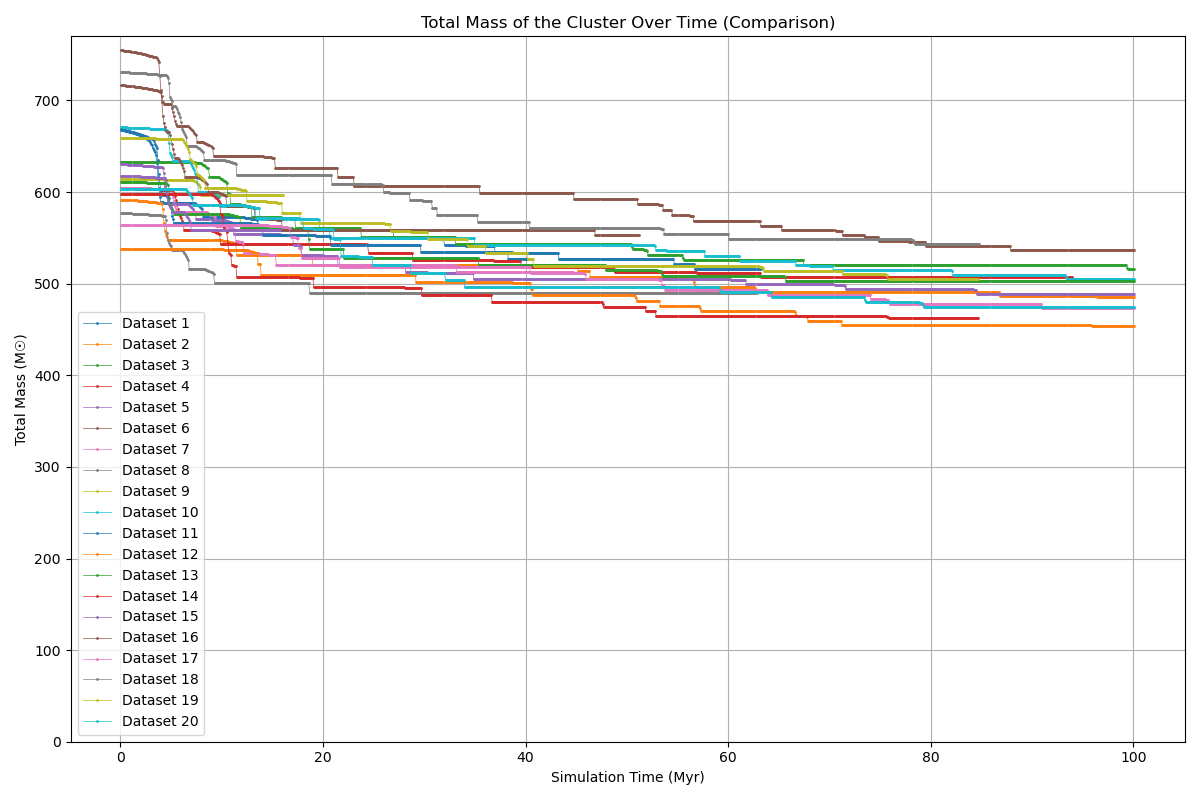
\includegraphics[width=\linewidth]{mass_comparison_over_time.png}
            \caption{Mass loss over time for 20 simulations with initial conditions $w_0$=7, N=1000 stars, T=100 Myr}
            \label{fig:mass_loss}
    \end{figure}

The density profile evolved as anticipated, with mass becoming less concentrated at the cluster center and more diffuse towards the outskirts. This outcome reflects the King model's influence on the initial conditions and the gradual redistribution of stars over time. Figure \ref{fig:density_profile} highlights this change, showing snapshots of the density profile at multiple stages of the simulation. The truncation radius, representing the cluster's outer boundary, also decreased progressively, consistent with stars being lost to the galactic tidal field. This supports theoretical predictions about the impact of external forces on cluster stability.


Visualizations created during the simulation provided additional insights into the cluster’s evolution. 3D animations of star positions clearly illustrated the gradual dispersion of stars as the simulation progressed. These animations, combined with the density profile data, helped visualize the dynamic redistribution of mass within the cluster, with stars moving outward and some escaping the system altogether. Such visualizations are useful for understanding the complex interplay between internal dynamics and external tidal forces, providing a clearer picture of the mechanisms driving the cluster's evolution.

A sample of raw data, including star-by-star positions, masses, and other relevant parameters, is available in the "finalruns" folder within the main repository of the project. This folder contains the outputs from the simulation, providing a detailed record of the cluster's evolution over time. The data is stored in CSV format, allowing for easy extraction and analysis of the individual star properties at each timestep. Researchers and developers can access these raw datasets to further explore the simulation results, conduct additional analyses, or compare the outcomes with other models and studies.

Despite these successes, several limitations and caveats merit discussion. First, while the simulation captures overall trends, it does not account for all possible dynamical processes, such as interactions with molecular clouds or detailed three-body encounters. These could influence cluster dynamics and lead to deviations from the simulated results. Second, the computational constraints limited the number of stars in the cluster to 1,000. While sufficient for demonstrating the methods, larger clusters may exhibit different evolutionary behaviors. Finally, the simplifications in the stellar evolution model, which relies on precomputed tracks, could omit subtleties in the evolution of certain star types.

\begin{figure}
    \centering
    \begin{subfigure}[b]{0.45\linewidth}
        \centering
        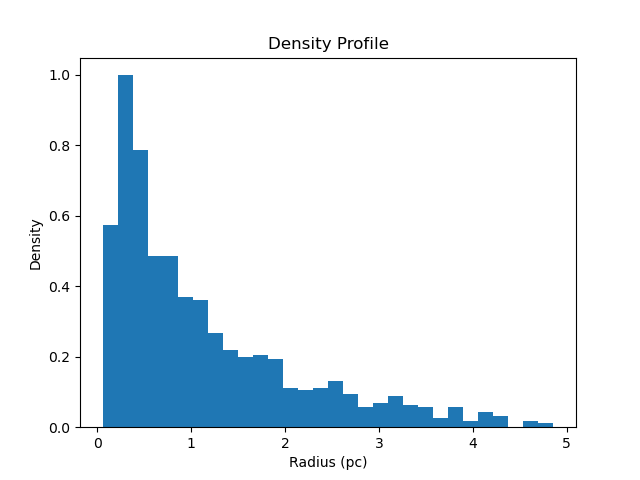
\includegraphics[width=\linewidth]{density_profile_initial.png}
        \caption{Initial Density Profile}
        \label{fig:sub1}
    \end{subfigure}
    \hfill
    \begin{subfigure}[b]{0.45\linewidth}
        \centering
        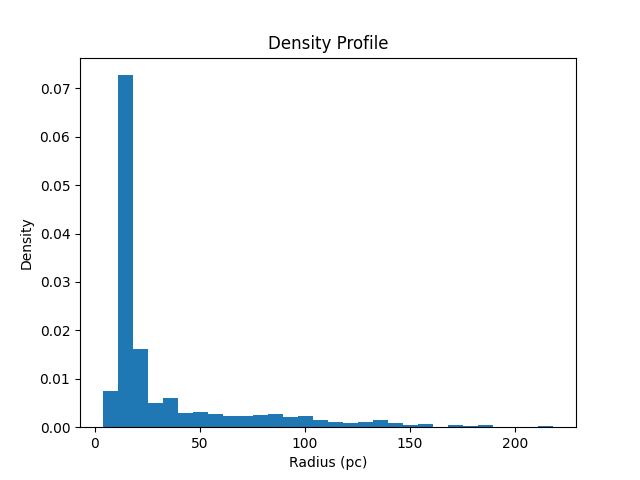
\includegraphics[width=\linewidth]{density_profile.png}
        \caption{Final Density Profile}
        \label{fig:sub2}
    \end{subfigure}
    \caption{Density profiles at the beginning and end of a run with initial conditions $w_0$=7, N=1000 stars, T=100 Myr.}
    \label{fig:density_profile}
\end{figure}


Future work will focus on addressing these limitations. Increasing the simulation scale and incorporating more complex dynamical interactions are necessary to enhance the realism of the results. Additionally, comparing the simulation outcomes to observed clusters and other computational models will help refine the approach and validate its accuracy. This discussion, along with the raw data provided in the project repository, offers a foundation for further analysis and development.

\section{Ethical Considerations}
Since this project focuses on simulating star clusters, the final product doesn’t have many direct societal or ethical implications. However, there are a few necessary ethical considerations when thinking about the process of the project. The accuracy and reliability of these models must be evaluated rigorously before they can be implemented towards any kind of research. Over-reliance on simulated results without validation against observational data can lead to misleading conclusions that might influence broader astrophysical research. Transparency about the limitations of these models, their assumptions, and approximations is essential to maintain scientific integrity.

Astrophysical simulations are computationally intensive and require significant energy resources, raising concerns about their environmental impact. The high-performance computing systems often used for such simulations consume large amounts of energy, which increases carbon emissions. Addressing this issue involves optimizing code efficiency, reducing unnecessary computational overhead, and leveraging renewable energy resources wherever possible.

The integration of artificial intelligence tools, such as AI-based coding assistants, also introduces important ethical questions. Generative artificial intelligence including OpenAI’s ChatGPT and Anthropic’s Claude large language models were used to generate and debug code, and occasionally to assist with the background research process. The use of AI can lead to concerns about plagiarism and intellectual property, as these tools often draw on publicly available databases to generate solutions. However, this project mostly used AI to debug code and to generate higher-level solutions to coding issues, and not enough code was copied and pasted directly from AI sources to raise concerns about intellectual property theft.

Another concern is bias within AI models. These tools are trained on vast datasets that may include inaccuracies or biases, as laid out in the seminal paper “On the Dangers of Stochastic Parrots” by Gebru et al.~\cite{gebru2021dangers}. Artificial intelligence can inadvertently propagate errors or reinforce stereotypical patterns in ways that are difficult to recognize or track. While astrophysics is less susceptible to such issues, reliance on AI tools might limit the diversity of approaches in problem-solving and coding. Excessive reliance on AI in coding may also reduce developers’ understanding of fundamental algorithms and implementations. This project mitigated this risk by using AI to supplement and debug code that was manually written after I gained a deeper understanding of the techniques used.

While AI has expanded research capabilities and improved efficiency, it also contributes to larger societal concerns such as job displacement, lack of algorithmic accountability, and technological inequity. These broader impacts highlight the importance of balancing AI’s benefits with its potential risks. Transparency about AI’s role in the research process, along with thorough documentation of its contributions, is vital to fostering responsible AI usage in scientific projects.

In summary, while this project does not engage directly with societal inequities or privacy issues, it is important to maintain a commitment to responsible scientific practices, careful management of computational resources, and critical engagement with AI tools in the coding process. Consideration of these topics throughout the process ensured that this project did not violate the principles of sustainability, integrity, and ethical responsibility in research.

\section{Timeline}

\subsection*{September}
The project was initiated due to a strong interest in simulations and astronomy, as well as an alignment with research conducted by Professor Sabrina Stierwalt at Occidental, to whom I reached out for help when I was first starting the project. Initial research focused on star clusters, their dynamics, and the tools used to model them. During this month, significant time was spent learning the AMUSE framework, which would form the foundation of the simulation. The project topic was not chosen until late August because I had previously planned to work on a project involving music and artificial intelligence, but I spent a lot of time this summer on computational modeling and simulation and decided to continue following those interests.

\subsection*{October}
In October, the primary focus shifted to writing code within the AMUSE framework. This involved developing the core simulation for modeling the gravitational dynamics and stellar evolution of star clusters. Alongside this, evaluation metrics were developed to assess the accuracy and performance of the simulation, focusing on mass loss, density profiles, and truncation radius. The simulation was finalized, and visualization code was created to enable the analysis of the data generated by the model.

\subsection*{November}
November was dedicated to preparing for the poster presentation, where key aspects of the project were summarized and visualized. During this time, the simulation was run to produce data for analysis. Minor tweaks were made to the final simulation, including adjustments to parameters and code optimization, ensuring that the project was ready for presentation.

\subsection*{December}
In December, the poster was presented, showcasing the results and methodology of the project. Writing the final paper began concurrently, documenting the entire process, results, and future directions. The simulation continued to run in the background, providing additional data for further analysis. The final paper was completed with a thorough discussion of the methods, results, and ethical considerations involved in the project.

\appendix

\section{Replication Instructions}

This section provides detailed instructions for replicating the simulation environment and executing the project to ensure future researchers can replicate and build upon the results.

\subsection{Overview of Software and Dependencies}
The project relies on the \textbf{Astrophysical Multipurpose Software Environment (AMUSE)} for simulations and several Python-based libraries for data analysis and visualization. All dependencies are specified with their respective versions to ensure compatibility. The recommended setup uses a virtual environment for package management to avoid conflicts with system-wide libraries.

\subsection{System Requirements}
The following system configuration is recommended for running the simulation:
\begin{itemize}
    \item \textbf{Operating System:} Ubuntu 20.04 LTS (or later), macOS 12.0+
    \item \textbf{Processor:} Multi-core CPU (2.5 GHz or faster)
    \item \textbf{Memory:} Minimum 8 GB RAM
    \item \textbf{Disk Space:} 10 GB of free storage
    \item \textbf{Python Version:} Python 3.9
\end{itemize}

\subsection{Installing Dependencies}
To install the necessary dependencies for the simulation, follow these steps:

\begin{itemize}
    \item \textbf{Install Python 3.9 and Pip}
       Ensure that Python 3.9 is installed. For Ubuntu, Python 3.9 and pip can be installed by using the package manager. On macOS, use Homebrew.
    \item \textbf{Set Up a Virtual Environment}
       It's recommended to create a Python virtual environment to keep the dependencies isolated. Use Python 3.9 to create the environment.
    \item \textbf{Install Required Libraries}
    \begin{itemize}
        \item AMUSE framework: Version 14.0
        \item AMUSE SeBa module: Version 14.0
        \item NumPy: Version 1.23.5
        \item Matplotlib: Version 3.7.0
        \item Pandas: Version 1.4.4
    \end{itemize}
\end{itemize}

\subsection{Cloning the Project Repository}
Clone the project’s GitHub repository to your local machine:
- Ensure you have git installed.
- Use the command to clone the repository.

\subsection{Running the Simulation}
To run the simulation, ensure the virtual environment is activated and execute the main Python script.

\subsection{Verifying Output}
After running the simulation, check the output directory for the following files:
- CSV files containing star positions and other data.
- Plots and graphs, such as the total mass over time and density profiles.

\subsection{Future-Proofing Notes}
For replicability, use \texttt{pip freeze > requirements.txt} to save the environment configuration and allow reinstallation with \texttt{pip install -r requirements.txt}.

\subsection{Troubleshooting}
If issues arise during installation or execution, consult the official AMUSE installation guide for troubleshooting tips. \\

By following these instructions, another researcher should be able to recreate the simulation environment and replicate the project results accurately.

\section{Appendix B: Code Architecture Overview}

This project is organized into three Python scripts, each serving a specific purpose in simulating, analyzing, and visualizing star cluster evolution. The modular design allows for easy debugging, extension, and reusability.

\subsection{Overview of Code Structure}

\textbf{(a) \texttt{newcluster.py}}: This script runs the primary simulation. It initializes a star cluster, simulates its evolution over time, and outputs data on star positions, masses, and other parameters. The results are stored in CSV files and visualized through plots.

\textbf{(b) \texttt{animaterun.py}}: This script processes the CSV files from a single simulation run, generating visualizations such as animations of star positions over time. It is focused on providing insight into the behavior of a single cluster evolution.

\textbf{(c) \texttt{chartmasses.py}}: This script analyzes multiple simulation runs, comparing trends like mass loss, density changes, and truncation radius across different runs. It is designed for large-scale comparative studies.

\subsection{\texttt{newcluster.py}: Simulation Script}
The \texttt{newcluster.py} script uses the \textbf{AMUSE} framework to simulate the gravitational and stellar evolution of a star cluster. 

\textbf{Core Components:}
\begin{itemize}
    \item \textbf{Initialization:} Sets up the cluster using a King model (\texttt{w0}) and the Kroupa initial mass distribution. The \texttt{Hermite} integrator computes gravitational interactions, while the \texttt{SeBa} module handles stellar evolution.
    \item \textbf{Simulation Loop:} Evolves the cluster over discrete time steps (\texttt{dt}) until the end time (\texttt{t\_end}). At each step:
    \begin{itemize}
        \item Gravitational and stellar evolution is calculated.
        \item Data on star positions, masses, and escape events are saved to CSV files.
        \item The truncation radius is recalculated based on density thresholds.
        \item Escaped stars are removed from the cluster.
    \end{itemize}
    \item \textbf{Outputs:} Generates CSV files for each time step, tracking star properties, and plots for metrics like total mass and density profiles.
\end{itemize}

\textbf{Extensibility:} 
\begin{itemize}
    \item Adding new physics modules, such as gas dynamics, is straightforward due to AMUSE’s modularity.
    \item Custom analysis methods can be incorporated into the loop by appending to the \texttt{evolve()} function.
\end{itemize}

\subsection{\texttt{animaterun.py}: Single-Run Analysis}
The \texttt{animaterun.py} script takes the CSV outputs from \texttt{newcluster.py} and creates animations and plots. 

\textbf{Key Features:}
\begin{itemize}
    \item Loads star position and mass data for a single run.
    \item Produces interactive 3D animations showing the evolution of star positions.
    \item Generates static plots such as the mass distribution and density profiles at specific time steps.
\end{itemize}

\textbf{Extensibility:}
\begin{itemize}
    \item Support for additional visualization methods, like heatmaps or velocity vectors, can be added by modifying the visualization functions.
\end{itemize}

\subsection{\texttt{chartmasses.py}: Multi-Run Comparison}
The \texttt{chartmasses.py} script compares the results of multiple simulation runs to identify trends and validate hypotheses. 

\textbf{Key Features:}
\begin{itemize}
    \item Loads and aggregates data from multiple simulation runs.
    \item Generates comparative plots, such as mass loss over time across different initial conditions.
    \item Computes summary statistics for metrics like truncation radius and star escape rates.
\end{itemize}

\textbf{Extensibility:}
\begin{itemize}
    \item Additional metrics, such as angular momentum or velocity dispersion, can be added by extending the data analysis pipeline.
\end{itemize}

\subsection{Justification for Design}
The separation of simulation, single-run analysis, and multi-run analysis improves modularity and maintainability:
\begin{itemize}
    \item \textbf{Debugging:} Errors can be isolated to specific scripts, making it easier to test and verify functionality.
    \item \textbf{Reusability:} The analysis scripts can be reused for simulations of other astrophysical systems, not just star clusters.
    \item \textbf{Collaboration:} Different team members can work on separate components without conflicts.
\end{itemize}

By following this architecture, other developers can easily extend, debug, or reuse components of this project.

\printbibliography

\end{document}